% Options for packages loaded elsewhere
\PassOptionsToPackage{unicode}{hyperref}
\PassOptionsToPackage{hyphens}{url}
\PassOptionsToPackage{dvipsnames,svgnames,x11names}{xcolor}
%
\documentclass[
  letterpaper,
  DIV=11,
  numbers=noendperiod]{scrreprt}

\usepackage{amsmath,amssymb}
\usepackage{iftex}
\ifPDFTeX
  \usepackage[T1]{fontenc}
  \usepackage[utf8]{inputenc}
  \usepackage{textcomp} % provide euro and other symbols
\else % if luatex or xetex
  \usepackage{unicode-math}
  \defaultfontfeatures{Scale=MatchLowercase}
  \defaultfontfeatures[\rmfamily]{Ligatures=TeX,Scale=1}
\fi
\usepackage[]{libertinus}
\ifPDFTeX\else  
    % xetex/luatex font selection
\fi
% Use upquote if available, for straight quotes in verbatim environments
\IfFileExists{upquote.sty}{\usepackage{upquote}}{}
\IfFileExists{microtype.sty}{% use microtype if available
  \usepackage[]{microtype}
  \UseMicrotypeSet[protrusion]{basicmath} % disable protrusion for tt fonts
}{}
\makeatletter
\@ifundefined{KOMAClassName}{% if non-KOMA class
  \IfFileExists{parskip.sty}{%
    \usepackage{parskip}
  }{% else
    \setlength{\parindent}{0pt}
    \setlength{\parskip}{6pt plus 2pt minus 1pt}}
}{% if KOMA class
  \KOMAoptions{parskip=half}}
\makeatother
\usepackage{xcolor}
\setlength{\emergencystretch}{3em} % prevent overfull lines
\setcounter{secnumdepth}{5}
% Make \paragraph and \subparagraph free-standing
\ifx\paragraph\undefined\else
  \let\oldparagraph\paragraph
  \renewcommand{\paragraph}[1]{\oldparagraph{#1}\mbox{}}
\fi
\ifx\subparagraph\undefined\else
  \let\oldsubparagraph\subparagraph
  \renewcommand{\subparagraph}[1]{\oldsubparagraph{#1}\mbox{}}
\fi

\usepackage{color}
\usepackage{fancyvrb}
\newcommand{\VerbBar}{|}
\newcommand{\VERB}{\Verb[commandchars=\\\{\}]}
\DefineVerbatimEnvironment{Highlighting}{Verbatim}{commandchars=\\\{\}}
% Add ',fontsize=\small' for more characters per line
\usepackage{framed}
\definecolor{shadecolor}{RGB}{241,243,245}
\newenvironment{Shaded}{\begin{snugshade}}{\end{snugshade}}
\newcommand{\AlertTok}[1]{\textcolor[rgb]{0.68,0.00,0.00}{#1}}
\newcommand{\AnnotationTok}[1]{\textcolor[rgb]{0.37,0.37,0.37}{#1}}
\newcommand{\AttributeTok}[1]{\textcolor[rgb]{0.40,0.45,0.13}{#1}}
\newcommand{\BaseNTok}[1]{\textcolor[rgb]{0.68,0.00,0.00}{#1}}
\newcommand{\BuiltInTok}[1]{\textcolor[rgb]{0.00,0.23,0.31}{#1}}
\newcommand{\CharTok}[1]{\textcolor[rgb]{0.13,0.47,0.30}{#1}}
\newcommand{\CommentTok}[1]{\textcolor[rgb]{0.37,0.37,0.37}{#1}}
\newcommand{\CommentVarTok}[1]{\textcolor[rgb]{0.37,0.37,0.37}{\textit{#1}}}
\newcommand{\ConstantTok}[1]{\textcolor[rgb]{0.56,0.35,0.01}{#1}}
\newcommand{\ControlFlowTok}[1]{\textcolor[rgb]{0.00,0.23,0.31}{#1}}
\newcommand{\DataTypeTok}[1]{\textcolor[rgb]{0.68,0.00,0.00}{#1}}
\newcommand{\DecValTok}[1]{\textcolor[rgb]{0.68,0.00,0.00}{#1}}
\newcommand{\DocumentationTok}[1]{\textcolor[rgb]{0.37,0.37,0.37}{\textit{#1}}}
\newcommand{\ErrorTok}[1]{\textcolor[rgb]{0.68,0.00,0.00}{#1}}
\newcommand{\ExtensionTok}[1]{\textcolor[rgb]{0.00,0.23,0.31}{#1}}
\newcommand{\FloatTok}[1]{\textcolor[rgb]{0.68,0.00,0.00}{#1}}
\newcommand{\FunctionTok}[1]{\textcolor[rgb]{0.28,0.35,0.67}{#1}}
\newcommand{\ImportTok}[1]{\textcolor[rgb]{0.00,0.46,0.62}{#1}}
\newcommand{\InformationTok}[1]{\textcolor[rgb]{0.37,0.37,0.37}{#1}}
\newcommand{\KeywordTok}[1]{\textcolor[rgb]{0.00,0.23,0.31}{#1}}
\newcommand{\NormalTok}[1]{\textcolor[rgb]{0.00,0.23,0.31}{#1}}
\newcommand{\OperatorTok}[1]{\textcolor[rgb]{0.37,0.37,0.37}{#1}}
\newcommand{\OtherTok}[1]{\textcolor[rgb]{0.00,0.23,0.31}{#1}}
\newcommand{\PreprocessorTok}[1]{\textcolor[rgb]{0.68,0.00,0.00}{#1}}
\newcommand{\RegionMarkerTok}[1]{\textcolor[rgb]{0.00,0.23,0.31}{#1}}
\newcommand{\SpecialCharTok}[1]{\textcolor[rgb]{0.37,0.37,0.37}{#1}}
\newcommand{\SpecialStringTok}[1]{\textcolor[rgb]{0.13,0.47,0.30}{#1}}
\newcommand{\StringTok}[1]{\textcolor[rgb]{0.13,0.47,0.30}{#1}}
\newcommand{\VariableTok}[1]{\textcolor[rgb]{0.07,0.07,0.07}{#1}}
\newcommand{\VerbatimStringTok}[1]{\textcolor[rgb]{0.13,0.47,0.30}{#1}}
\newcommand{\WarningTok}[1]{\textcolor[rgb]{0.37,0.37,0.37}{\textit{#1}}}

\providecommand{\tightlist}{%
  \setlength{\itemsep}{0pt}\setlength{\parskip}{0pt}}\usepackage{longtable,booktabs,array}
\usepackage{calc} % for calculating minipage widths
% Correct order of tables after \paragraph or \subparagraph
\usepackage{etoolbox}
\makeatletter
\patchcmd\longtable{\par}{\if@noskipsec\mbox{}\fi\par}{}{}
\makeatother
% Allow footnotes in longtable head/foot
\IfFileExists{footnotehyper.sty}{\usepackage{footnotehyper}}{\usepackage{footnote}}
\makesavenoteenv{longtable}
\usepackage{graphicx}
\makeatletter
\def\maxwidth{\ifdim\Gin@nat@width>\linewidth\linewidth\else\Gin@nat@width\fi}
\def\maxheight{\ifdim\Gin@nat@height>\textheight\textheight\else\Gin@nat@height\fi}
\makeatother
% Scale images if necessary, so that they will not overflow the page
% margins by default, and it is still possible to overwrite the defaults
% using explicit options in \includegraphics[width, height, ...]{}
\setkeys{Gin}{width=\maxwidth,height=\maxheight,keepaspectratio}
% Set default figure placement to htbp
\makeatletter
\def\fps@figure{htbp}
\makeatother

\KOMAoption{captions}{tableheading}
\makeatletter
\@ifpackageloaded{bookmark}{}{\usepackage{bookmark}}
\makeatother
\makeatletter
\@ifpackageloaded{caption}{}{\usepackage{caption}}
\AtBeginDocument{%
\ifdefined\contentsname
  \renewcommand*\contentsname{Table of contents}
\else
  \newcommand\contentsname{Table of contents}
\fi
\ifdefined\listfigurename
  \renewcommand*\listfigurename{List of Figures}
\else
  \newcommand\listfigurename{List of Figures}
\fi
\ifdefined\listtablename
  \renewcommand*\listtablename{List of Tables}
\else
  \newcommand\listtablename{List of Tables}
\fi
\ifdefined\figurename
  \renewcommand*\figurename{Figure}
\else
  \newcommand\figurename{Figure}
\fi
\ifdefined\tablename
  \renewcommand*\tablename{Table}
\else
  \newcommand\tablename{Table}
\fi
}
\@ifpackageloaded{float}{}{\usepackage{float}}
\floatstyle{ruled}
\@ifundefined{c@chapter}{\newfloat{codelisting}{h}{lop}}{\newfloat{codelisting}{h}{lop}[chapter]}
\floatname{codelisting}{Listing}
\newcommand*\listoflistings{\listof{codelisting}{List of Listings}}
\makeatother
\makeatletter
\makeatother
\makeatletter
\@ifpackageloaded{caption}{}{\usepackage{caption}}
\@ifpackageloaded{subcaption}{}{\usepackage{subcaption}}
\makeatother
\ifLuaTeX
  \usepackage{selnolig}  % disable illegal ligatures
\fi
\usepackage{bookmark}

\IfFileExists{xurl.sty}{\usepackage{xurl}}{} % add URL line breaks if available
\urlstyle{same} % disable monospaced font for URLs
\hypersetup{
  pdftitle={Ichthyop User Guide},
  pdfauthor={Nicolas Barrier},
  colorlinks=true,
  linkcolor={blue},
  filecolor={Maroon},
  citecolor={Blue},
  urlcolor={Blue},
  pdfcreator={LaTeX via pandoc}}

\title{Ichthyop User Guide}
\author{Nicolas Barrier}
\date{}

\begin{document}
\maketitle

\renewcommand*\contentsname{Table of contents}
{
\hypersetup{linkcolor=}
\setcounter{tocdepth}{2}
\tableofcontents
}
\bookmarksetup{startatroot}

\chapter*{Preface}\label{preface}
\addcontentsline{toc}{chapter}{Preface}

\markboth{Preface}{Preface}

\bookmarksetup{startatroot}

\chapter{Getting started}\label{getting-started}

In this section, download and install instructions are provided.

\section{Prerequisites}\label{prerequisites}

\subsection{Java}\label{java}

In order to run Ichthyop, \textbf{Java (\textgreater= 11)} needs to be
installed. Beforehand, let us clarify some of the acronyms regarding the
Java technologies.

\{samp\}\texttt{JVM}: Java Virtual Machine. It is a set of software
programs that interprets the Java byte code.

\{samp\}\texttt{JRE}: Java Runtime Environment. It is a kit distributed
by Sun to execute Java programs. A \{samp\}\texttt{JRE} provides a
\{samp\}\texttt{JVM} and some basic Java libraries.

\{samp\}\texttt{JDK} or \{samp\}\texttt{SDK}: Java (or Software)
Development Kit bound to the programmer. It provides a
\{samp\}\texttt{JRE}, a compiler, useful programs, examples and the
source of the API (Application Programming Interface: some standard
libraries).

It is strongly recommended to download a \{samp\}\texttt{JDK}, in order
to both compile and run the model. Builds for different platforms can be
found \href{https://www.oracle.com/java/technologies/downloads/}{here}.

(nc-inst)=

\subsection{NetCDF4}\label{netcdf4}

The Java library that manages input/outputs of NetCDF files requires the
external NetCDF C library, which can be installed as follows:

\subsubsection{Mac Os X}\label{mac-os-x}

To install the library on a Mac Os system, open a Terminal and type:

\begin{Shaded}
\begin{Highlighting}[]
\FunctionTok{sudo}\NormalTok{ port install netcdf4}
\end{Highlighting}
\end{Shaded}

\subsubsection{Linux}\label{linux}

To install the library on a Linux system, open a Terminal and type:

\begin{Shaded}
\begin{Highlighting}[]
\FunctionTok{sudo}\NormalTok{ apt{-}get install netcdf4}
\end{Highlighting}
\end{Shaded}

\subsubsection{Windows}\label{windows}

To install the library on a Windows system, download the pre-built
libraries ib
\href{https://docs.unidata.ucar.edu/netcdf-c/current/winbin.html}{Unidata
website}

During the install process, make sure that the location of the library
is added to the \{samp\}\texttt{PATH}

\subsection{Conda environmenmt}\label{conda-environmenmt}

There also is the possibility to use Conda environments in order to
install Maven, OpenJDK and NetCDF4 easily. Instructions can be found on
\url{https://github.com/ichthyop/ichthyop-conda}

\section{Downloading Ichthyop}\label{sec-osm-inst}

The Ichthyop model is available on
\href{https://github.com/ichthyop/ichthyop}{GitHub}. There is two ways
to recover Ichthyop:

\begin{itemize}
\tightlist
\item
  Using executable files (\texttt{.jar} files).
\item
  From source files.
\end{itemize}

\subsection{Using executables}\label{using-executables}

Ichthyop users can download Ichthyop executables
\href{https://github.com/ichthyop/ichthyop/releases}{here}. Choose a
version, and download the
\{samp\}\texttt{ichthyop-X.Y.Z-jar-with-dependencies.jar} file
(replacing \{samp\}\texttt{X.Y.Z} by the version number).

\subsection{From source}\label{from-source}

To get the source code, type in a Terminal (Unix/MacOs) or Git Bash
prompt (Windows):

\begin{Shaded}
\begin{Highlighting}[]
\FunctionTok{git}\NormalTok{ clone https://github.com/ichthyop/ichthyop.git}
\end{Highlighting}
\end{Shaded}

The code can then be compiled either using IDE (NetBeans, VSCode) or
using the following command line:

\begin{Shaded}
\begin{Highlighting}[]
\ExtensionTok{mvn}\NormalTok{ package}
\end{Highlighting}
\end{Shaded}

The executable will be generated in the \texttt{target} folder.

To use the command line, Maven needs to be installed (see instructions
on \url{https://maven.apache.org/install.html})

\section{Running Ichthyop}\label{running-ichthyop}

\subsection{Clicking on file (Windows)}\label{clicking-on-file-windows}

Open the Ichthyop folder and double click on the
\texttt{ichthyop-X.Y.Z-jar-with-dependencies.jar} file, where
\texttt{X.Y.Z} is the Ichthyop version. You should see the Ichthyop
console.

\subsection{From command line (Unix/Mac Os
X)}\label{from-command-line-unixmac-os-x}

Open a command line prompt (Terminal or CMD prompt) and navigate to the
Ichthyop folder using \texttt{cd}.

Then, type:

\begin{Shaded}
\begin{Highlighting}[]
\ExtensionTok{java} \AttributeTok{{-}jar}\NormalTok{ ichthyop{-}X.Y.Z{-}jar{-}with{-}dependencies.jar}
\end{Highlighting}
\end{Shaded}

with \texttt{X.Y.Z} the Ichthyop version.

This will prompt the Java console. In order to run Ichthyop without the
console, you need to specify a supplementary argument, which is the XML
configuration file.

\begin{Shaded}
\begin{Highlighting}[]
\ExtensionTok{java} \AttributeTok{{-}jar}\NormalTok{ ichthyop{-}X.Y.Z{-}jar{-}with{-}dependencies.jar cfg{-}roms3d.xml}
\end{Highlighting}
\end{Shaded}

\bookmarksetup{startatroot}

\chapter{Ichthyop configuration}\label{ichthyop-configuration}

\section{Simulation configuration file}\label{sec-xml-config}

Ichthyop simulations are configured using
\href{https://en.wikipedia.org/wiki/XML}{XML} configuration files. It
should always start as follows:

\begin{Shaded}
\begin{Highlighting}[]
\NormalTok{\textless{}}\KeywordTok{icstructure}\NormalTok{\textgreater{}}
\NormalTok{\textless{}}\KeywordTok{long\_name}\NormalTok{\textgreater{}Generic Ichthyop configuration file\textless{}/}\KeywordTok{long\_name}\NormalTok{\textgreater{}}
\NormalTok{\textless{}}\KeywordTok{description}\NormalTok{\textgreater{}The file has few pre{-}defined parameters.\textless{}/}\KeywordTok{description}\NormalTok{\textgreater{}}

\NormalTok{\textless{}/}\KeywordTok{icstructure}\NormalTok{\textgreater{}}
\end{Highlighting}
\end{Shaded}

\subsection{Configuration blocks}\label{configuration-blocks}

Ichthyop is configured by blocks, each block managing a specific aspect
of the model. The blocks are as follows:

\begin{itemize}
\tightlist
\item
  \texttt{ACTION}: Block of parameters related to the \texttt{action}
  classes (cf.~\{numref\}\texttt{process}).
\item
  \texttt{RELEASE}: Block of parameters related to the \texttt{release}
  classes (cf.~\{numref\}\texttt{release})
\item
  \texttt{DATASET}: Block of parameters related to the \texttt{datasets}
  classes.
\item
  \texttt{OPTION}: Block of parameters related to the remaining
  parameters.
\end{itemize}

New blocks can be added in the XML file as follows:

\begin{Shaded}
\begin{Highlighting}[]
\NormalTok{\textless{}}\KeywordTok{block}\OtherTok{ type=}\StringTok{"option"}\NormalTok{\textgreater{}}
\NormalTok{        \textless{}}\KeywordTok{key}\NormalTok{\textgreater{}app.transport\textless{}/}\KeywordTok{key}\NormalTok{\textgreater{}}
\NormalTok{        \textless{}}\KeywordTok{enabled}\NormalTok{\textgreater{}true\textless{}/}\KeywordTok{enabled}\NormalTok{\textgreater{}}
\NormalTok{        \textless{}}\KeywordTok{tree\_path}\NormalTok{\textgreater{}Transport/General\textless{}/}\KeywordTok{tree\_path}\NormalTok{\textgreater{}}
\NormalTok{        \textless{}}\KeywordTok{description}\NormalTok{\textgreater{}Set the general transport options of the simulation.\textless{}/}\KeywordTok{description}\NormalTok{\textgreater{}}
\NormalTok{\textless{}/}\KeywordTok{block}\NormalTok{\textgreater{}}
\end{Highlighting}
\end{Shaded}

The \texttt{key} tag is used to identify the configuration block. The
\texttt{tree\_path} tag is used in the Ichthyop console to create the
parameter tree. The \texttt{description} field is used to display the
block description in the Ichthyop console.

The \texttt{enabled} tag specifies whether the block should be
considered by Ichthyop or not. By default, all blocks are enabled. But
for the \texttt{RELEASE} and \texttt{DATASET}, one and only one block
must be activated.

\subsection{Configuration parameters}\label{configuration-parameters}

To each block is associated a list of parameters. This list of parameter
is added in the XML as follows:

\begin{Shaded}
\begin{Highlighting}[]
\NormalTok{\textless{}}\KeywordTok{parameters}\NormalTok{\textgreater{}}
\NormalTok{\textless{}/}\KeywordTok{parameters}\NormalTok{\textgreater{}}
\end{Highlighting}
\end{Shaded}

Inside the \texttt{parameters} tags, new parameters are defined as
follows:

\begin{Shaded}
\begin{Highlighting}[]
\NormalTok{\textless{}}\KeywordTok{parameter}\NormalTok{\textgreater{}}
\NormalTok{    \textless{}}\KeywordTok{key}\NormalTok{\textgreater{}output\_path\textless{}/}\KeywordTok{key}\NormalTok{\textgreater{}}
\NormalTok{    \textless{}}\KeywordTok{value}\NormalTok{\textgreater{}output\textless{}/}\KeywordTok{value}\NormalTok{\textgreater{}}
\NormalTok{    \textless{}}\KeywordTok{long\_name}\NormalTok{\textgreater{}Output path\textless{}/}\KeywordTok{long\_name}\NormalTok{\textgreater{}}
\NormalTok{    \textless{}}\KeywordTok{format}\NormalTok{\textgreater{}path\textless{}/}\KeywordTok{format}\NormalTok{\textgreater{}}
\NormalTok{    \textless{}}\KeywordTok{default}\NormalTok{\textgreater{}output\textless{}/}\KeywordTok{default}\NormalTok{\textgreater{}}
\NormalTok{    \textless{}}\KeywordTok{description}\NormalTok{\textgreater{}Select the folder where the simulation NetCDF output file should be saved.\textless{}/}\KeywordTok{description}\NormalTok{\textgreater{}}
\NormalTok{\textless{}/}\KeywordTok{parameter}\NormalTok{\textgreater{}}
\end{Highlighting}
\end{Shaded}

The \texttt{key} tag allows to identify the parameter, while the
\texttt{value} tag specifies the value of the parameter. The remaining
tags are only used by the Ichthyop console. The \texttt{long\_name} and
\texttt{description} tags are used by the console to provide
informations about the parameter.

The \texttt{format} tag specifies the parameter format, which will be
used by the console parameter editor. The accepted values are:

\begin{itemize}
\tightlist
\item
  \texttt{path}: For files and folders
\item
  \texttt{date}: For dates (format must be
  \texttt{year\ YYYY\ month\ MM\ day\ at\ HH:MM})
\item
  \texttt{duration}: For duration (format must be
  \texttt{\#\#\#\#\#\#\ day(s)\ \#\#\#\ hour(s)\ \#\#\#\ minute(s)})
\item
  \texttt{float}: For real values
\item
  \texttt{integer}: For integer values.
\item
  \texttt{class}: For class parameters. It allow the user to choose an
  existing Ichthyop class in the configuration file.
\item
  \texttt{list}: For a list of string parameters, separated by
  \texttt{,}
\item
  \texttt{boolean}: For boolean parameters. It allows the user to select
  \texttt{true} or \texttt{false} using a simple combo box.
\item
  \texttt{combo}: For parameters with a limited set of values, which can
  be selected in the console with a combo box.
\item
  \texttt{lonlat}: For geographical coordinates.
\end{itemize}

In the case of \texttt{combo} parameters, the list of accepted
parameters is specified by providing as many \texttt{accepted} tags as
necessary. For instance:

\begin{Shaded}
\begin{Highlighting}[]
\NormalTok{\textless{}}\KeywordTok{parameter}\NormalTok{\textgreater{}}
\NormalTok{    \textless{}}\KeywordTok{key}\NormalTok{\textgreater{}time\_arrow\textless{}/}\KeywordTok{key}\NormalTok{\textgreater{}}
\NormalTok{    \textless{}}\KeywordTok{long\_name}\NormalTok{\textgreater{}Direction of the simulation\textless{}/}\KeywordTok{long\_name}\NormalTok{\textgreater{}}
\NormalTok{    \textless{}}\KeywordTok{value}\NormalTok{\textgreater{}forward\textless{}/}\KeywordTok{value}\NormalTok{\textgreater{}}
\NormalTok{    \textless{}}\KeywordTok{format}\NormalTok{\textgreater{}combo\textless{}/}\KeywordTok{format}\NormalTok{\textgreater{}}
\NormalTok{    \textless{}}\KeywordTok{accepted}\NormalTok{\textgreater{}backward\textless{}/}\KeywordTok{accepted}\NormalTok{\textgreater{}}
\NormalTok{    \textless{}}\KeywordTok{accepted}\NormalTok{\textgreater{}forward\textless{}/}\KeywordTok{accepted}\NormalTok{\textgreater{}}
\NormalTok{    \textless{}}\KeywordTok{default}\NormalTok{\textgreater{}forward\textless{}/}\KeywordTok{default}\NormalTok{\textgreater{}}
\NormalTok{    \textless{}}\KeywordTok{description}\NormalTok{\textgreater{}Run the simulation backward or forward in time.\textless{}/}\KeywordTok{description}\NormalTok{\textgreater{}}
\NormalTok{\textless{}/}\KeywordTok{parameter}\NormalTok{\textgreater{}}
\end{Highlighting}
\end{Shaded}

If a parameter should appear as hidden in the Ichthyop console, it can
be specified by adding the \texttt{hidden="true"} argument to the
\texttt{parameter} tag, as shown below:

\begin{Shaded}
\begin{Highlighting}[]
\NormalTok{\textless{}}\KeywordTok{parameter}\OtherTok{ hidden=}\StringTok{"true"}\NormalTok{\textgreater{}}
\NormalTok{\textless{}/}\KeywordTok{parameter}\NormalTok{\textgreater{}}
\end{Highlighting}
\end{Shaded}

\subsection{Serial parameters}\label{serial-parameters}

In order to test different values for a given parameter, a
\texttt{serial} tag can be added as follows:

\begin{Shaded}
\begin{Highlighting}[]
\NormalTok{\textless{}}\KeywordTok{parameter}\OtherTok{ type=}\StringTok{"serial"}\NormalTok{\textgreater{}}
\NormalTok{\textless{}/}\KeywordTok{parameter}\NormalTok{\textgreater{}}
\end{Highlighting}
\end{Shaded}

Different values are provided by replicating the \texttt{value}
parameter as follows:

\begin{Shaded}
\begin{Highlighting}[]
\NormalTok{\textless{}}\KeywordTok{parameter}\OtherTok{ type=}\StringTok{"serial"}\NormalTok{\textgreater{}}
\NormalTok{  \textless{}}\KeywordTok{key}\NormalTok{\textgreater{}initial\_time\textless{}/}\KeywordTok{key}\NormalTok{\textgreater{}}
\NormalTok{  \textless{}}\KeywordTok{long\_name}\NormalTok{\textgreater{}Beginning of simulation\textless{}/}\KeywordTok{long\_name}\NormalTok{\textgreater{}}
\NormalTok{  \textless{}}\KeywordTok{value}\NormalTok{\textgreater{}year 2001 month 10 day 20 at 00:00\textless{}/}\KeywordTok{value}\NormalTok{\textgreater{}}
\NormalTok{  \textless{}}\KeywordTok{value}\NormalTok{\textgreater{}year 2001 month 10 day 21 at 00:00\textless{}/}\KeywordTok{value}\NormalTok{\textgreater{}}
\NormalTok{  \textless{}}\KeywordTok{format}\NormalTok{\textgreater{}date\textless{}/}\KeywordTok{format}\NormalTok{\textgreater{}}
\NormalTok{  \textless{}}\KeywordTok{description}\NormalTok{\textgreater{}Set the beginning date and time of the simulation. Format: year \#\#\#\#\#\# month \#\#\# day \#\#\# at HH:mm.\textless{}/}\KeywordTok{description}\NormalTok{\textgreater{}}
\NormalTok{\textless{}/}\KeywordTok{parameter}\NormalTok{\textgreater{}}
\end{Highlighting}
\end{Shaded}

\textbf{Using the GUI, additionnal values can be provided to serial
parameters only when hidden parameters are displayed}

When simulations are run with serial parameters, all possible
combinations of parameters will be run. Output files will contain a
\texttt{\_sX} suffix, with \texttt{X} the simulation number. The
parameters used in the simulation are provided as global NetCDF
attributes.

\section{Zone configuration file}\label{sec-zone-xml-config}

Zone configuration files are also managed via a dedicated XML file. The
file must be as follows:

\begin{Shaded}
\begin{Highlighting}[]
\FunctionTok{\textless{}?xml}\OtherTok{ version=}\StringTok{"1.0"}\OtherTok{ encoding=}\StringTok{"UTF{-}8"}\FunctionTok{?\textgreater{}}
\NormalTok{\textless{}}\KeywordTok{zones}\NormalTok{\textgreater{}}

\NormalTok{\textless{}/}\KeywordTok{zones}\NormalTok{\textgreater{}}
\end{Highlighting}
\end{Shaded}

Each zone is defined on a \texttt{zone} tag, which contain the following
tags:

\begin{itemize}
\tightlist
\item
  \texttt{key} is the name of the zone
\item
  \texttt{enabled} specifies whether this zone must be considered or
  not.
\item
  \texttt{type} specifies whether the zone should be used for release
  (see :numref:\texttt{,\ \textasciigrave{}\textasciigrave{}release}
  value) or recruitment processes (\texttt{recruitment} value)
\item
  \texttt{polygon} specifies the different points used to define the
  area
\item
  \texttt{bathy\_mask} specifies the bathymetric zone (for instance 0 to
  200m, i.e.~continental shelf) where the zone is defined.
\item
  \texttt{thickness} specifies the upper and lower depths where this
  zone is defined (\textbf{only valid for 3D runs}).
\item
  \texttt{color} specifies the display color of the zone (format is
  \texttt{{[}r=102,g=51,b=255{]}}).
\item
  \texttt{proportion\_particles} specifies the proportion (values in
  \([0-1]\)) of particles to be released in the area. Only used when
  \texttt{type} is \texttt{release} and if the
  \texttt{user\_defined\_nparticles} parameter is set to True
  (cf.~\{numref\}\texttt{zone-release})
\end{itemize}

An example of a zone definition is provided below.

\begin{Shaded}
\begin{Highlighting}[]
\NormalTok{\textless{}}\KeywordTok{zone}\NormalTok{\textgreater{}}
\NormalTok{    \textless{}}\KeywordTok{key}\NormalTok{\textgreater{}Release zone 2\textless{}/}\KeywordTok{key}\NormalTok{\textgreater{}}
\NormalTok{    \textless{}}\KeywordTok{enabled}\NormalTok{\textgreater{}true\textless{}/}\KeywordTok{enabled}\NormalTok{\textgreater{}}
\NormalTok{    \textless{}}\KeywordTok{type}\NormalTok{\textgreater{}release\textless{}/}\KeywordTok{type}\NormalTok{\textgreater{}}
\NormalTok{    \textless{}}\KeywordTok{polygon}\NormalTok{\textgreater{}}
\NormalTok{        \textless{}}\KeywordTok{point}\NormalTok{\textgreater{}}
\NormalTok{            \textless{}}\KeywordTok{index}\NormalTok{\textgreater{}0\textless{}/}\KeywordTok{index}\NormalTok{\textgreater{}}
\NormalTok{            \textless{}}\KeywordTok{lon}\NormalTok{\textgreater{}54.0\textless{}/}\KeywordTok{lon}\NormalTok{\textgreater{}}
\NormalTok{            \textless{}}\KeywordTok{lat}\NormalTok{\textgreater{}{-}11.5\textless{}/}\KeywordTok{lat}\NormalTok{\textgreater{}}
\NormalTok{        \textless{}/}\KeywordTok{point}\NormalTok{\textgreater{}}
\NormalTok{        \textless{}}\KeywordTok{point}\NormalTok{\textgreater{}}
\NormalTok{            \textless{}}\KeywordTok{index}\NormalTok{\textgreater{}1\textless{}/}\KeywordTok{index}\NormalTok{\textgreater{}}
\NormalTok{            \textless{}}\KeywordTok{lon}\NormalTok{\textgreater{}54.0\textless{}/}\KeywordTok{lon}\NormalTok{\textgreater{}}
\NormalTok{            \textless{}}\KeywordTok{lat}\NormalTok{\textgreater{}{-}12.5\textless{}/}\KeywordTok{lat}\NormalTok{\textgreater{}}
\NormalTok{        \textless{}/}\KeywordTok{point}\NormalTok{\textgreater{}}
\NormalTok{        \textless{}}\KeywordTok{point}\NormalTok{\textgreater{}}
\NormalTok{            \textless{}}\KeywordTok{index}\NormalTok{\textgreater{}2\textless{}/}\KeywordTok{index}\NormalTok{\textgreater{}}
\NormalTok{            \textless{}}\KeywordTok{lon}\NormalTok{\textgreater{}53.0\textless{}/}\KeywordTok{lon}\NormalTok{\textgreater{}}
\NormalTok{            \textless{}}\KeywordTok{lat}\NormalTok{\textgreater{}{-}12.5\textless{}/}\KeywordTok{lat}\NormalTok{\textgreater{}}
\NormalTok{        \textless{}/}\KeywordTok{point}\NormalTok{\textgreater{}}
\NormalTok{        \textless{}}\KeywordTok{point}\NormalTok{\textgreater{}}
\NormalTok{            \textless{}}\KeywordTok{index}\NormalTok{\textgreater{}3\textless{}/}\KeywordTok{index}\NormalTok{\textgreater{}}
\NormalTok{            \textless{}}\KeywordTok{lon}\NormalTok{\textgreater{}53.0\textless{}/}\KeywordTok{lon}\NormalTok{\textgreater{}}
\NormalTok{            \textless{}}\KeywordTok{lat}\NormalTok{\textgreater{}{-}11.5\textless{}/}\KeywordTok{lat}\NormalTok{\textgreater{}}
\NormalTok{        \textless{}/}\KeywordTok{point}\NormalTok{\textgreater{}}
\NormalTok{    \textless{}/}\KeywordTok{polygon}\NormalTok{\textgreater{}}
\NormalTok{    \textless{}}\KeywordTok{bathy\_mask}\NormalTok{\textgreater{}}
\NormalTok{        \textless{}}\KeywordTok{enabled}\NormalTok{\textgreater{}true\textless{}/}\KeywordTok{enabled}\NormalTok{\textgreater{}}
\NormalTok{        \textless{}}\KeywordTok{line\_inshore}\NormalTok{\textgreater{}0.0\textless{}/}\KeywordTok{line\_inshore}\NormalTok{\textgreater{}}
\NormalTok{        \textless{}}\KeywordTok{line\_offshore}\NormalTok{\textgreater{}12000.0\textless{}/}\KeywordTok{line\_offshore}\NormalTok{\textgreater{}}
\NormalTok{    \textless{}/}\KeywordTok{bathy\_mask}\NormalTok{\textgreater{}}
\NormalTok{    \textless{}}\KeywordTok{thickness}\NormalTok{\textgreater{}}
\NormalTok{        \textless{}}\KeywordTok{enabled}\NormalTok{\textgreater{}true\textless{}/}\KeywordTok{enabled}\NormalTok{\textgreater{}}
\NormalTok{        \textless{}}\KeywordTok{upper\_depth}\NormalTok{\textgreater{}0.0\textless{}/}\KeywordTok{upper\_depth}\NormalTok{\textgreater{}}
\NormalTok{        \textless{}}\KeywordTok{lower\_depth}\NormalTok{\textgreater{}50.0\textless{}/}\KeywordTok{lower\_depth}\NormalTok{\textgreater{}}
\NormalTok{        \textless{}/}\KeywordTok{thickness}\NormalTok{\textgreater{}}
\NormalTok{    \textless{}}\KeywordTok{color}\NormalTok{\textgreater{}[r=102,g=51,b=255]\textless{}/}\KeywordTok{color}\NormalTok{\textgreater{}}
\NormalTok{    \textless{}}\KeywordTok{proportion\_particles}\NormalTok{\textgreater{}0.2\textless{}/}\KeywordTok{proportion\_particles}\NormalTok{\textgreater{}}
\NormalTok{\textless{}/}\KeywordTok{zone}\NormalTok{\textgreater{}}
\end{Highlighting}
\end{Shaded}

\section{Time configuration}\label{sec-time-config}

\subsection{Beginning of the
simulation}\label{beginning-of-the-simulation}

In Ichthyop, the user provides the time at which the simulation should
start. This \texttt{initial\_time} parameter, which must be defined in
the \texttt{app.time} option block, must be formatted as
\texttt{year\ YYYY\ month\ MM\ day\ DD\ at\ HH:MM}, with \texttt{YYYY}
the year, \texttt{MM} the month, \texttt{DD} the day, \texttt{HH} the
hour and \texttt{MM} the minutes where the simulation should start.

\subsection{Reading NetCDF times}\label{reading-netcdf-times}

When reading a NetCDF file (ocean currents, temperature, wind, wave,
etc.), Ichthyop will determine the units in which NetCDF time is stored.
These units must meet the
\href{https://cfconventions.org/Data/cf-conventions/cf-conventions-1.7/build/ch04s04.html}{CF
Metadata Conventions} and therefore be provided as follows:

\begin{Shaded}
\begin{Highlighting}[]
\ExtensionTok{UNITS}\NormalTok{ since YYYY{-}MM{-}DD HH:MM:SS}
\end{Highlighting}
\end{Shaded}

with \texttt{UNITS} the units in which the time is stored (usually
\texttt{seconds}, \texttt{days} or \texttt{hours}), \texttt{YYYY} the
year, \texttt{MM} the month, \texttt{DD} the day, \texttt{HH} the hour,
\texttt{MM} the minutes and \texttt{SS} the seconds of the reference
date.

If a NetCDF \texttt{time::units} attribute is defined, Ichthyop will try
to infer the NetCDF reference date and time units using this convention.

If it fails (i.e.~the \texttt{time::units} attribute does not follow the
convention) or if no \texttt{time::units} attribute is found, Ichthyop
will read the \texttt{time\_origin} parameter from the \texttt{app.time}
option block, which must be defined following the CF conventions.

When reading two datasets (an ocean currents dataset and a wind dataset
for instance), if none meets the CF convention, Ichthyop will apply the
units defined in the \texttt{time\_origin} parameter to both datasets,
even though they may have different time units. \textbf{Therefeore, in
this case, it is strongly recommended to manually include CF-like time
units attributes to each dataset (cf.~below).}

Manually updating the \texttt{units} attribute can be done by using the
\href{https://linux.die.net/man/1/ncatted}{ncatted} command
(\textbf{Linux users}):

\begin{Shaded}
\begin{Highlighting}[]
\CommentTok{\#!/bin/bash}
\ControlFlowTok{for}\NormalTok{ file }\KeywordTok{in} \PreprocessorTok{*}\NormalTok{nc}
\ControlFlowTok{do}
    \ExtensionTok{ncatted} \AttributeTok{{-}O} \AttributeTok{{-}a}\NormalTok{ units,time,o,s,}\StringTok{"seconds since 1900{-}01{-}01 00:00:00"} \VariableTok{$file}
\ControlFlowTok{done}
\end{Highlighting}
\end{Shaded}

This can also be done by using Python as follows:

\begin{Shaded}
\begin{Highlighting}[]
\ImportTok{from}\NormalTok{ glob }\ImportTok{import}\NormalTok{ glob}
\ImportTok{import}\NormalTok{ xarray }\ImportTok{as}\NormalTok{ xr}

\NormalTok{units }\OperatorTok{=} \StringTok{\textquotesingle{}seconds since 1900{-}01{-}01 00:00:00\textquotesingle{}}
\NormalTok{time }\OperatorTok{=} \StringTok{\textquotesingle{}time\textquotesingle{}}

\NormalTok{filelist }\OperatorTok{=}\NormalTok{ glob(}\StringTok{\textquotesingle{}*nc\textquotesingle{}}\NormalTok{)}

\ControlFlowTok{for}\NormalTok{ f }\KeywordTok{in}\NormalTok{ filelist:}

\NormalTok{    data }\OperatorTok{=}\NormalTok{ xr.open\_dataset(f)}
\NormalTok{    data[time].attrs[}\StringTok{\textquotesingle{}units\textquotesingle{}}\NormalTok{] }\OperatorTok{=}\NormalTok{ units}
\NormalTok{    data[time]}

\NormalTok{    data.to\_netcdf(f)}
\end{Highlighting}
\end{Shaded}

The user must replace \texttt{time} by the name of the time variable
which is used by Ichthyop. Common values are \texttt{time},
\texttt{scrum\_time}, \texttt{time\_counter}, \texttt{ocean\_time}.

The units value must also be chosen consistently with the dataset

\bookmarksetup{startatroot}

\chapter{Ichthyop console}\label{sec-console}

In this section, the Ichthyop console is described.

\section{Configuration}\label{configuration}

Here you will find the usual ``File menu'' functions : create a new
configuration file, open an existing one, close it or save and save as
the configuration file.

\begin{figure}

\centering{

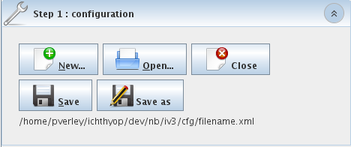
\includegraphics{_static/step1-configure.png}

}

\caption{\label{fig-elephant}Step 1, configure}

\end{figure}%

\subsection{New configuration file}\label{new-configuration-file}

:::\{figure\} \_static/new.png :align: center

Step 1, create a new configuration file :::

The application comes with some preset examples of configuration files
(the templates). Select one of the templates, change the name of the
configuration if the suggested name does not suit you and click on the
Create button.

\subsection{Content of the configuration
file}\label{content-of-the-configuration-file}

:::\{figure\} \_static/edit.png :align: center

Step 1, edit the configuration file :::

The configuration file is organized in several categories and each
category contains several blocks of parameters.

When the configuration file is created out of a template, it is ready to
use and you do not need to change any parameter for running the
simulation. Little by little you can explore the configuration file,
starting with the ``Main'' blocks and change some parameters to see what
is happening. On a second time you can start playing with the advanced
parameters that activate and control the behaviors of the particles.

Main blocks:

\begin{itemize}
\tightlist
\item
  Time: Set the simulation time options, such as the beginning of the
  simulation, the duration of transport, the time step, etc.
\item
  Output: Options that control the record of the particle tracks in a
  NetCDF output file.
\item
  Dataset: Management of the hydrodynamic dataset.
\item
  Release: Determine how and where the particles should be released.
\end{itemize}

Advanced blocks:

\begin{itemize}
\tightlist
\item
  Transport: Parameters for controlling the advection process, the
  dispersion, the vertical migration, the wind drift, etc.
\item
  Release: Additional ways for releasing particles, from zones, with
  position recorded in a text file or in a NetDCF file, etc.
\item
  Biology: Control the biological processes such as growth or cold water
  sensitivity, etc.
\end{itemize}

Each block is fully described and commented in the block information
area. As well, you will find a description and the necessary
explanations for each parameter in the parameter information area.

Do not forget to save the configuration file before going to the next
step.

\textbf{Parameters cannot be added from within the Ichthyop console.
Only paramters that are already defined on the XML file can be edited
using the console}

\section{Zone definition}\label{zone-definition}

In Ichthyop, the user can define zones, either release zones or
recruitment zones.

The zones can be edited using the GUI, as shown in
\{numref\}\texttt{figure-gui-zone}

(figure-gui-zone)=

:::\{figure\} \_static/zone.png :align: center :width: 600px

Ichthyop Zone editor :::

\subsection{Adding, removing and renaming
zones}\label{adding-removing-and-renaming-zones}

The number of zones is managed on the left part of the panel.

New zones can be added by clicking the \{\{ listadd \}\} button. When a
zone is selected, it can be removed by clicking on the \{\{ listremove
\}\} button.

The reordering of the zones is achieved by clicking on the \{\{ up \}\}
and \{\{ down \}\} buttons.

When double-clicking on the name of the zone on the left panel, the user
can edit the zone name.

\subsection{Editing a zone}\label{editing-a-zone}

When a zone is selected, the user can edit different parameters
associated with the zone.

First, the user can enable or disable a zone by clicking on the
\{guilabel\}\texttt{Enabled} tick box.

The zones are defined by providing the points coordinates. Points can be
added, removed and reordered by using the \{\{ listadd \}\}, \{\{
listremove \}\}, \{\{ up \}\} and \{\{ down \}\} buttons, respectively.
The user can also change the format of the points coordinates by
clicking on the radio buttons in the \{guilabel\}\texttt{Options} bottom
panel.

Ichthyop defines two types of zones: one for release (see
\{numref\}\texttt{zone-release}) problèmeand one for recruitment
purposes. This type is chosen by using the
\{guilabel\}\texttt{Type\ of\ zone} combo box. For release zones, the
user can specify the number of particles that will be released in the
zone (only if the \texttt{user\_defined\_nparticles} parameter is set
equal to true, cf \{numref\}\texttt{zone-release}). It is done by
filling the \{guilabel\}\texttt{Number\ of\ released\ particles} textbox
and pressing \{guilabel\}\texttt{ENTER}

Each zone is associated with a color, that will be used to its
representation in the graphical interface during the preview and the
display of the simulation results. This color can be edited by using the
\{\{ color \}\} button.

In the case of 3D simulations, you can specify the depth range to use in
the zone. To activate this feature, click on the
\{guilabel\}\texttt{Activated} tick box of the
\{guilabel\}\texttt{Thickness} panel. You can provide the lower and
upper depth that must be considered in the given zone (negative values).

In 3D simulations, you can also specify the bathymetric range that you
want to include, for instance if you want to release particles only on
the ocean shelf (i.e depth less than 200m). This can be done by
activating the feature by clicking on the \{samp\}\texttt{Activated}
tick box of the \{guilabel\}\texttt{Bathymetric\ mask} panel.

\section{Running}\label{running}

:::\{figure\} \_static/step2-simulate.png :align: center

Step 2, simulation :::

You may want to preview the simulated area. Click on the ``Preview''
button. The main interest in previewing the area is that the application
will check if the simulation is correctly set up. Here ``correctly''
does not mean you made a relevant parametrization in terms of physics or
biology, but at least the application had found all the parameters
required for starting the simulation. More specifically, Ichthyop will
attempt to read the geographical variables (longitude, latitude and
depth) from the dataset in order to draw the area. It should also
display the release and the recruitment zones if they have been defined
and activated in the configuration file. Make sure what you see is what
you expect, and go back to ``Step 1: configure'' in case not.

When the preview is satisfactory, click on ``Run simulation'' for
starting the simulation. The progress bar will give an estimation of the
remaining time for the simulation to complete. You can interrupt (but
not pause) the simulation anytime by a click on ``Stop simulation''.

Depending the capabilities of your computer, the number of released
particles, how many actions are implemented, etc. the simulation might
requires a large amount of the available dynamic memory and the
application might look like it is frozen. Wait until the simulation run
to completion. Refer to section ``Java Heap Space'' if the application
crashes because of memory problem.

\bookmarksetup{startatroot}

\chapter{Visualize results}\label{visualize-results}

:::\{figure\} \_static/step3-mapping.png :align: center

Step 3, mapping :::

When the simulation is completed, the application automatically opens
the current Ichthyop output file for visualizing the results. If your
computer is connected to Internet, you should see the map being centered
above the simulated area. Otherwise, it only displays a Grey background.

You may want to skip that step or keep it for later. In that case, just
click on ``Close NetCDF'' and go to any other steps or exit the
application. Any time, you can go back to this step: click on ``Open
NetCDF'' and select the Ichthyop output file you wish to visualize. When
the NetCDF file is opened, the application brings you back to the exact
point where it was when the simulation just completed.

The application offers two ways for visualizing the results : draw the
particle trajectories with a Web Map Service or export the particle
trajectories in a KMZ file that can be opened with Google Earth. Both
functions are completely independent one from another.

\section{Results}\label{results}

Ichthyop archives the particle trajectories in NetCDF format, a
machine-independent data formats for sharing array-oriented scientific
data. The NetDCF file is recorded in the output folder (set in the
Output section of the configuration file) and the file name contains the
date and time of creation of the file.

Default contents of the NetCDF output file: time of the simulation,
longitude, latitude, and depth at particle position, and mortality
status.

\section{Set particle color}\label{set-particle-color}

The \{guilabel\}\texttt{Default\ color} button determines the particle
color for visualizing the trajectories.

Particles are plotted as small circles.
\{guilabel\}\texttt{Particle\ size} determines the diameter of the
circle in pixel.

To use a colorbar, select in the Combo box a variable archived in the
Ichthyop output file you wish to visualize as a tri-color range. The
:guilabel`Auto range` button will scan the values of the variable and
suggest the following range : {[}mean - 2 * standard deviation; mean + 2
* standard deviation{]}. Do not forget to click on
\{guilabel\}\texttt{Apply\ settings} for validating the changes of the
color bar.

For taking off the color bar, select the :guilabel`None` item in the
Combo box and click on :guilabel`Apply settings`. A click on
:guilabel`Default color` button should also deactivate the color bar.

\section{Make maps using Web Map
Service}\label{make-maps-using-web-map-service}

According to Wikipedia, a Web Map Service (WMS) is a standard protocol
for serving georeferenced map images over the Internet.

Ichthyop provides three different WMS for displaying the ocean
bathymetry and the cost line as a background of the particle
trajectories.

Maps can be intuitively zoomed in and out with the mouse wheel and
re-centered doing a mere drag and drop.

Depending on the quality of the Internet connection and how busy is the
Web Map Server, the display of the background tiles might take a while
or even not work at all. In that case, try again with a distinct WMS and
change the zoom scale.

When the settings of the map looks satisfactory, click on ``Make maps''
button. Ichthyop will create a folder that has exactly the same name
than the simulation NetCDF output file (without the .nc extension) in
the output directory. Then maps are recorded in this folder as PNG
pictures.

Again, depending on the computer capabilities and the number of
particles, the map creation might require a large amount of the
available dynamic memory and the application looks like it is frozen.
Wait for the application to complete this step. Refer to section ``Java
Heap Space'' if the application crashes because of memory problem.

\section{Export trajectories to KMZ
format}\label{export-trajectories-to-kmz-format}

By default, Ichthyop records the particle trajectories in NetCDF format.
It is perfectly adapted for archiving and sharing scientific data since
it is a machine independent and array-oriented format. But it is not
much handy for visualizing results.

Click on ``Export to KMZ'' button for recording the particle
trajectories into a KMZ file. The file is recorded in the same directory
than the Ichthyop output file, with the same name and the ``.kmz''
extension. KMZ format is the standard file format for visualizing
georeferenced information with GoogleEarth.

Color settings (default color or color bar) and particle size will also
be stored in the KMZ file.

When the export has performed, browse to the output folder and click on
the KMZ file for launching GoogleEarth (assuming the program is
installed on your computer).

\section{Animation}\label{animation}

Here you will find the usual ``File menu'' functions : create a new
configuration file, open an existing one, close it or save and save as
the configuration file.

:::\{figure\} \_static/step4-animation.png :align: center

Step 4, Animation :::

You may want to skip that step or keep it for later. In that case, just
go to any other steps or exit the application. Any time, you can go back
to this step, click on ``Open maps'' and select the simulation output
folder that contains the PNG pictures you wish to visualize. When the
folder is opened, the application brings you back to the exact point
where it was when the map creation just completed.

Set the number of frames per second of the animation with the spinner.

You can also create an animated GIF. The file is recorded in the same
directory than the Ichthyop output file, with the same name and the
``.gif'' extension.



\end{document}
